\documentclass{standalone}
\usepackage{chez}

\begin{document}
\chapter{October 09, 2020}

\subsection{Summary}
If \(X\) is a CW complex, then \(\Ccell_*(X)\) is a chain complex
with homology groups computing the singular homology groups \(H_q(X)\).
The \(n\)th group \(\Ccell_n(X)\) is the free abelian group on the
set \(I_n\) of \(n\)-cells. To compute the differential
\(d \colon \Ccell_n(X) \to \Ccell_{n-1}(X)\),
we consider the diagram
\[
  \begin{tikzcd}
    \coprod_{i \in I_n} S^{n-1} \arrow[r] \arrow[d] &
      \Sk_{n-1} X \arrow[d] \arrow[r] &
      \Sk_{n-1} X / \Sk_{n-2} X
        \mathrlap{{} \iso \bigvee_{i \in I_{n-1}} S^{n-1}} \\
    \coprod_{i \in I_n} D^n \arrow[r] &
       \Sk_n X
  \end{tikzcd}
\]
Applying \(H_{n-1}\) to the top row,
\(d \colon \Ccell_n(X) \to \Ccell_{n-1}(X)\).

If \(f \colon X \to Y\) is a map in \(\cTop\),
then to compute \(H_q(f) \colon H_q(X) \to H_q(Y)\),
We can place CW structures on \(X\) and \(Y\) so that
\(f\) induces a map \(\Ccell_*(X) \to \Ccell_*(Y)\).

\subsection{Homology of real projective space}
Recall \(\RP^n \coloneq S^n / (x \sim -x)\).
To compute the homology of this, we may try to do this by
coming up with a semisimplicial model for this space,
but it is not obvious how to do this.

However, we do have a CW structure on \(\RP^n\),
with one \(k\)-cell in each dimension \(0 \leq k \leq n\).
We can try to determine \(H_q(\RP^2)\).
Consider the pushout square
\[
  \begin{tikzcd}[row sep=small]
    S^1 \arrow[r] \arrow[d] &
      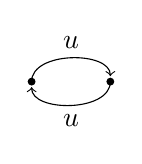
\begin{tikzpicture}[yshift=0.6ex]
        \fill (-1/2, 0) circle (0.05);
        \fill (1/2, 0) circle (0.05);
        \path[->, shorten >=2] (-1/2, 0) edge[in=90, out=90] node[above] {\(u\)} (1/2, 0);
        \path[<-, shorten <=2] (-1/2, 0) edge[in=-90, out=-90] node[below] {\(u\)} (1/2, 0);
      \end{tikzpicture} \arrow[d] \arrow[r, "\text{quotient}"] &
      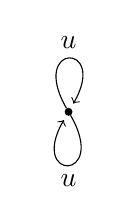
\begin{tikzpicture}
        \fill (0, 0) circle (0.05);
        \path[->, shorten >=2] (120: 0.05) edge[in=60, out=120, looseness=50] node[above] {\(u\)} (60: 0.05);
        \path[->, shorten >=2] (-60: 0.05) edge[in=-120, out=-60, looseness=50] node[below] {\(u\)} (-120: 0.05);
      \end{tikzpicture}
      \mathrlap{{} \iso S^1} \\
    D^2 \arrow[r] &
      \RP^2
  \end{tikzcd}
\]
Taking \(H_1\) of the top row, we have a map \(\ZZ \to \ZZ\).
More specifically, the \(2\)-cell gets mapped to \(u^2\),
so the map is \(1 \mapsto 2\).
We have the chain \(\Ccell_*(\RP^2)\)
\[
   \begin{tikzcd}[row sep=0.2]
  	0 \ar[r] &
      \ZZ\fgen{A} \ar[r] &
      \ZZ\fgen{u} \ar[r] &
      \ZZ\fgen{x} \\
    & A \ar[r, mapsto] &
      2u \\
    & & u \ar[r, mapsto] &
      0
  \end{tikzcd}
\]
This gives
\[
  H_0(\RP^2) \iso \ZZ, \qquad
  H_1(\RP^2) \iso \ZZ / 2\ZZ, \qquad
  H_2(\RP^2) \iso 0.
\]
This is a bit weird. Usually our homologies are free abelian groups.
Here, this means that there is some loop that is not a boundary,
but when we go around it twice, it is a boundary.

Now let's consider \(\Ccell_*(\RP^n)\) in general.
Let's try to think about this inductively.
If we understand \(\Ccell_*(\RP^{n-1})\),
can we say anything about \(\Ccell_*(\RP^{n})\)?
Consider the pushout diagram
\[
  \begin{tikzcd}
    S^{n-1} \arrow[r] \arrow[d] &
      \RP^{n-1} \arrow[d] \arrow[r] &
      \RP^{n-1} / \RP^{n-2} \mathrlap{{} \iso S^{n-1}} \\
    D^n \arrow[r] &
      \RP^n
  \end{tikzcd}
\]
Note that the way that we can think about \(\RP^{n-1} / \RP^{n-2}\)
is to take \(S^{n-1} \vee S^{n-1}\) and quotient by the antipodal map
between the two spheres.
The differential \(d\) maps \(1\) to \(1 + \deg f\),
where \(f\) is antipodal map \(S^{n-1} \to S^{n-1}\).
This is because the top half of the first \(S^{n-1}\)
gets mapped to \(S^{n-1}\), and the bottom half
gets mapped to the second \(S^{n-1}\), but under the quotient
this is equal to the antipodal map of the identity.
Therefore, \(d \colon 1 \mapsto 1 + (-1)^n\).

This gives the chain
\[
  \Ccell_*(\RP^n) \iso \Big(
  \begin{tikzcd}
  	\cdots \ar[r] &
  	0 \ar[r] &
  	\ZZ \ar[r] &
  	\cdots \ar[r] &
  	\ZZ \ar[r, "2"] &
  	\ZZ \ar[r, "0"] &
  	\ZZ \ar[r, "2"] &
  	\ZZ \ar[r, "0"] &
  	\ZZ
  \end{tikzcd}
  \Big),
\]
where the number of \(\ZZ\)s in the chain is \(n+1\).
In general, this means for even \(n\),
\[
  H_q(\RP^n) = \begin{cases*}
    \ZZ & \(q = 0\) \\[-1ex]
    \ZZ/2\ZZ & \(0 < q < n\), odd \(q\) \\[-1ex] % chktex 1
    0 & otherwise
  \end{cases*}
\]
and for odd \(n\),
\[
  H_q(\RP^n) = \begin{cases*}
    \ZZ & \(q = 0, n\) \\[-1ex]
    \ZZ/2\ZZ & \(0 < q < n\), odd \(q\) \\[-1ex] % chktex 1
    0 & otherwise.
  \end{cases*}
\]

\section{Other invariants}
Let's talk about other invariants that give strictly less information
than homology. The advantage is that they are easier to compute than homology.

\begin{definition}
  If \(X\) is a finite CW complex,
  then the \vocab{Euler characteristic} is
  \[
    \chi(X) = \sum_k (-1)^k \size{I_k}.
  \]
\end{definition}

\begin{example}
  Consider \(S^2\) with one \(0\)-cell and one \(2\)-cell.
  The Euler characteristic is \(\chi(S^2) = 1 + 1 = 2\).

  There is the other CW structure with two \(0\)-cells,
  \(1\)-cells, and \(2\)-cells.
  This gives the Euler characteristic \(\chi(S^2) = 2 - 2 + 2 = 2\).
\end{example}

\begin{theorem}
  The Euler characteristic \(\chi(X)\) depends only on
  the homotopy type of \(X\).
\end{theorem}

\begin{example}
  Consider the torus \(T^2\) with the CW structure
  from \cref{ex:torus-cell-homology}.
  This gives us the Euler characteristic
  \(\chi(T^2) = 1 - 2 + 1 = 0\).

  A corollary of this is that \(T^2\) and \(S^2\)
  are not homotopy equivalent.
\end{example}

\begin{theorem}
  If \(X\) is a finite CW complex, then
  \[
    \chi(X) = \sum_k (-1)^k \rank H_k(X).
  \]
\end{theorem}
To define rank, recall that abelian groups are equivalent to \(\ZZ\)-modules.
Since \(\ZZ\) is a PID, there is a classification of finitely generated
abelian groups. In particular, every finitely generated abelian group \(A\)
is isomorphic to
\[
  \ZZ^r \oplus \ZZ/n_1\ZZ \oplus \dots \oplus \ZZ/n_t\ZZ
\]
where \(r \geq 0\) and \(n_1, \dots, n_t \geq 2\).
We call \(r\) the \vocab{rank} of \(A\).

Note that since \(X\) is a finite CW complex, we know that \(H_k(X)\)
is finitely generated for each \(k\).







\end{document}
